\paragraph{La classe Dispatcher}

\begin{minipage}
    {\linewidth}
    \centering
    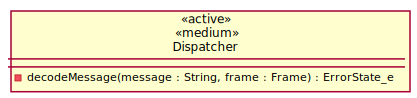
\includegraphics[width=0.55\linewidth]{../schemas/Conception_detaillee/classe_dispatcher.pdf}
    \captionof{figure}{Diagramme de classe de Dispatcher}
\end{minipage}

\subparagraph{Philosophie de conception \newline} 

\medspace

La classe Dispatcher a pour rôle de lire et décoder les trames et les demandes d'états du Mode Envoi reçu. Ces informations sont sous forme de chaînes de caractères lors de leur réception par la classe Dispatcher. Il transmet les trames décodées à la classe Sender.

\subparagraph{Description structurelle \newline}

\medspace

\textbf{Attributs :}

N.A.

\textbf{Services offerts :}

\begin{itemize}
    \item \textbf{decodeMessage(message : String, frame : Frame) : ErrorState\_e} --- Opération qui décode une chaîne de caractères en une structure représentant une trame à envoyer sur le réseau CAN. Permet également le décodage des demandes d'état du Mode Envoi.
\end{itemize}
